\documentclass[12pt,a4paper,twopage]{article}
\usepackage[utf8]{inputenc}
\usepackage[a4paper,margin=1cm,footskip=.5cm]{geometry}
\usepackage{multicol}
\usepackage{amsmath}
\usepackage{float}
\usepackage{epsfig,graphicx}
\usepackage{xcolor,import}
\usepackage{subcaption}
\usepackage[font=small,labelfont=bf]{caption}
\usepackage{siunitx}
\usepackage[german]{babel}
\usepackage{textcomp}
\usepackage{mathtools}
\linespread{1.1}
\usepackage{parskip}
%\setlength{\parskip}{14pt}
\setlength{\parindent}{12pt}

\begin{document}

\begin{verbatim}


\end{verbatim}
\begin{verbatim}


\end{verbatim}

\thispagestyle{empty}
			\begin{center}
			\Large{Fakultät für Physik}\\
			\end{center}
\begin{verbatim}


\end{verbatim}
							%Eintrag des Wintersemesters
			\begin{center}
			\textbf{\LARGE SOMMERSEMESTER 2015}
			\end{center}
\begin{verbatim}


\end{verbatim}
			\begin{center}
			\textbf{\LARGE{Physikalisches Praktikum II}}
			\end{center}
\begin{verbatim}




\end{verbatim}

			\begin{center}
			\textbf{\LARGE{PROTOKOLL}}
			\end{center}
			
\begin{verbatim}





\end{verbatim}

			\begin{flushleft}
			\textbf{\Large{Experiment (Nr. 6, Strahlung)}}\\
							%Experiment Nr. und Titel statt den Punkten eintragen
			\LARGE{}	
			\end{flushleft}

\begin{verbatim}

\end{verbatim}	
							%Eintragen des Abgabedatums, oder des Erstelldatums des Protokolls
			\begin{flushleft}
			\textbf{\Large{Datum:}} \Large{8.5.2015}
			\end{flushleft}
			
\begin{verbatim}
\end{verbatim}
							%Namen der Protokollschreiber
		\begin{flushleft}
			\textbf{\Large{Bachleitner Veronika, Grafendorfer Erik}} 
			\end{flushleft}

\begin{verbatim}


\end{verbatim}
							%Kurstag und Gruppennummer, zb. Fr/5
			\begin{flushleft}
			\textbf{\Large{Kurstag/Gruppe:}} \Large{FR/1}
			\end{flushleft}

\begin{verbatim}

\end{verbatim}
							%Name des Betreuers, das Praktikum betreute.
			\begin{flushleft}
			\LARGE{\textbf{Betreuer:\Large{ Jürgen KLEPP }}}		
			\end{flushleft}
\newpage
\begin{verbatim}


\end{verbatim}
			
\section{Aufgabenstellung}
Wir untersuchen die Interaktion elektromagnetischer Strahlung mit Materie an zwei unterschiedlichen Effekten - dem fotoelektrischen Effekt und der Schwarzkörperstrahlung.
\section{Theorie}
\subsection{Planck'sches Wirkungsquantum}
Beim Fotoeffekt werden elektrisch geladene Teilchen aus Materie angeregt (in einen höheren Energiezustand gebracht) oder freigesetzt, wenn sie von elektromagnetischen Wellen bestrahlt wird. 

Bei der Anregung spricht man vom \textit{Inneren Fotoeffekt}, bei Freisetzung von Elektronen vom \textit{Äußeren Fotoeffekt}. Letzteres kommt bei Metallen vor, bei denen man die Leitungselektronen als frei in einem Potentialtopf beweglich beschreiben kann. Werden sie mit Energie größer gleich der notwendigen Austrittsarbeit angeregt, können die Elektronen sich aus dem Metall lösen. Die zusätzliche Energie wird zur kinetischen Energie der Elektronen.\\
\\
Einstein-Formel:
$$h\cdot\nu=A+E_{kin}=A+\frac{mv^2}{2}=A+eU_0$$
Daraus können wir umformen:
$$U_0=\frac{h\cdot\nu}{e} - \frac{A}{e}$$
Diese Gleichung werden wir später verwenden, um $h$ und $A$ zu berechnen.


\subsection{Wärmestrahlung}
Das Planck'sche Strahlungsgesetz ist wie folgt gegeben:
\begin{equation}
L(\lambda,T)d\lambda = \frac{2hc^2}{\lambda^5} \cdot \frac{1}{\exp\left(\frac{hc}{\lambda kT}\right) -1} d\lambda
\label{strahlungsgesetz}
\end{equation}
wo $L(\lambda,T)d\lambda$ die gerichtete spektrale Strahldichte, abhängig von Wellenlänge und Temperatur. $L$ hat die Einheit $\frac{W}{m^2}\frac{sr}{nm}$.\\
\\

\begin{align}
\label{waermetheorie}
\frac{P_1}{P_2}& = \frac{T_1^4}{T_2^4} \\
\ln \frac{I_1}{I_2} &= \frac{1}{T_1} \left(\sqrt[4]{\frac{P_1}{P_2}}-1\right) \cdot \frac{ch}{k\lambda} \\
\frac{I_1}{I_2} &= \frac{r_1^2}{r_2^2}
\label{waermeende}
\end{align}

wo $P_i$ die zugeführte elektrische Leistung und $T_i$ die Temperatur, 
$I_i$ die Lichtstärken und $r_i$ die Abstände von der Lichtquelle bedeuten.
Hier machen wir noch auf einen Fehler in der Aufgabenstellung aufmerksam: Dort war $\frac{I_1}{I_2} = \frac{r_2^2}{r_1^2}$ angegeben, richtig ist aber $\frac{I_1}{I_2} = \frac{r_1^2}{r_2^2}$, wie man an folgender Herleitung sieht:


\begin{align*}
E&=\frac{I}{r^2}\\
E_1&= E_ 2 \\
\Rightarrow \frac{I_1}{r_1^2}&= \frac{I_2}{r_2^2} \\
\Rightarrow I_1&= \frac{I_2 \cdot \textbf{$r_1^2$}}{r_2^2} \\
\Rightarrow \frac{I_1}{I_2}&= \frac{r_1^2}{r_2^2}
\end{align*}

Schließlich formen wir all diese Gleichungen zu einem Ausdruck für $T_1$ um:
\begin{equation}
T_1=\frac{1}{ln \frac{I_1}{I_2}}\cdot \left( \sqrt[4]{\frac{P_1}{P_2}-1} \right) \cdot \frac{c\cdot h}{k_B\cdot \lambda}
\end{equation} 
\section{Aufbau}
\subsection{Planck'sches Wirkungsquantum}
Für den Versuch verwenden wir eine Gegenfeld-Kompensationsschaltung: In einem Stromkreis befinden sich eine Kathode (Metallplatte) und ein Anodenring, an dem eine Gegenspannung angelegt werden kann.\\
Vor einer Quecksilberdampflampe werden Frequenzfilter eingespannt, um die gewünschten Frequenzen zu bekommen. Die Photonen treffen auf die Kathode, aus der aufgrund des Fotoeffekts Elektronen herausgeschlagen werden. Wandern diese Elektronen zur Anode können wir Strom messen. Bei Anlegung einer Gegenspannung am Anodenring sehen wir, wann die schnellsten Elektronen nicht mehr ankommen.

\subsection{Wärmestrahlung}
Für den Versuch verwenden wir eine Glühlampe, einen Interferenzfilter (um monochromatisches Licht zu erzeugen, $\lambda=560\si{nm}$ und eine Fotozelle. Außerdem einen Strom-Spannungswandler, um den in der Fotozelle erzeugten Strom messen zu können.

\section{Durchführung}
\subsection{Planck'sches Wirkungsquantum}
Wir machen ungefähr 10 Messungen des Stroms an der Fotokathode mit einem Pikoamperemeter, wobei wir bei jeder Messung die Gegenspannung mit einem Potentiometer variieren. Diese 10 Messungen machen wir jeweils für Licht aus einem von fünf Interferenzfiltern.  

Durch lineare Extrapolation der Spannungsabhängigkeit des Stroms können wir auf die Gegenspannung $U_0$ und dadurch also auf die kinetische Energie der Elektronen schließen ($eU_0$). Damit erhalten wir über die Einstein-Formel das Planck'sche Wirkungsquantum und die Austrittsarbeit.

\subsection{Wärmestrahlung}
Wir messen die Spannung an einem Fotosensor für verschiedene Abstände des Sensors von einer Glühlampe, die in zwei unterschiedlichen Betriebsmodi glüht. Dabei machen wir für jeden Abstand eine Messung der Spannung, und messen dann für die gleichen Abstände beim zweiten Betriebsmodus. Für jeden Betriebsmodus messen wir weiterhin die elektrische Leistung an der Glühlampe.

 Wir plotten anschließend die der Lichtintensität proportionalen Spannungen am Fotosensor gegen das Inverse der Abstandsquadrate und erhalten natürlich ansteigende Geraden. Durch das Verhältnis der Anstiege dieser Geraden bekommen wir einen Ausdruck aus dem wir, gemeinsam mit den gemessenen Leistungen, auf die Temperaturen des Glühfadens in den unterschiedlichen Modi schließen können.

\section{Ergebnisse}
\subsection{Planck'sches Wirkungsquantum}
%Messen Sie den Fotostrom I als Funktion der Gegenspannung U im Bereich von 0-2V für fünf verschiedene Frequenzen und stellen Sie I gegen U in einem Diagramm graphisch dar.
%Führen Sie die Messung mit jedem der beiliegenden fünf dielektrischen Interferenzfilter durch. 
%Tragen Sie $\sqrt{I-I_0}$ gegen $U$ auf und extrapolieren Sie eine Gerade zum Schnittpunkt mit der U-Achse. Lesen Sie die damit eindeutig definierte Gegenspannung $U_0$ ab.

\begin{table}[H]
\begin{center}
\begin{tabular}{|c|l|}
\hline
$\nu$ ($10^{14}$Hz) & $U_0$ (V)\\
\hline
$5.187$ & $0.26 \pm 0.05$\\
$5.521$ & $0.27 \pm 0.03$\\
$6.908$ & $0.54 \pm 0.01$\\
$7.366$ & $0.58 \pm 0.01$\\
$8.213$ & $0.77 \pm 0.02$\\
\hline
\end{tabular}
\caption{Spannung $U_0$ zu den verschiedenen Frequenzfiltern.}
\end{center}
\end{table}

Wir zeigen ausführlich die Berechnung bei der Frequenz $\nu=5.187 \cdot 10^{14}\si{Hz}$
\begin{center}
\begin{figure}[H]
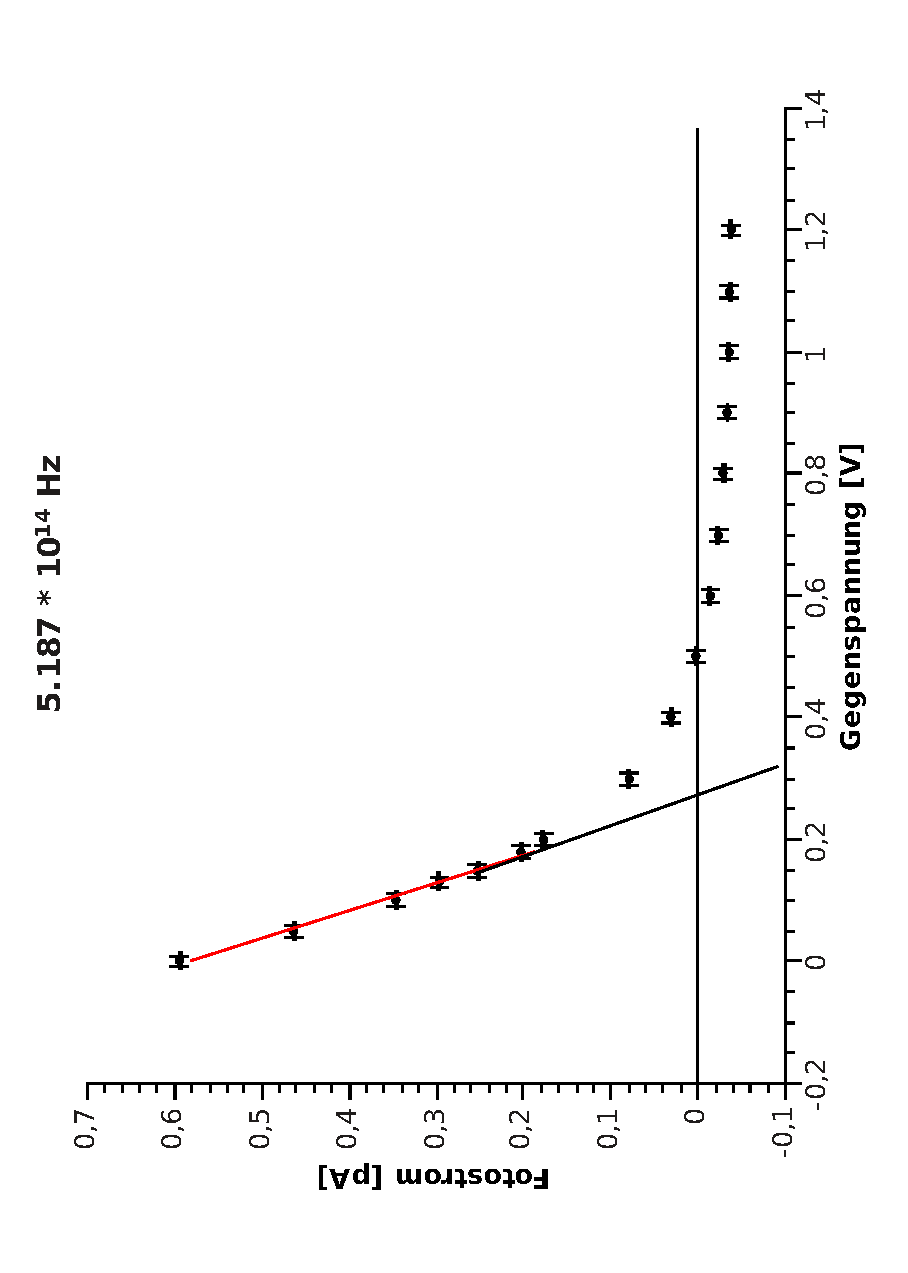
\includegraphics[scale=0.7, angle=-90]{5187.eps}
\caption{Datenpunkte und linearer Fit zur Frequenz $\nu=5.187 \cdot 10^{14}\si{Hz}$. Linearer Fit extrapoliert zum Schnittpunkt mit der U-Achse.}
\end{figure}
\end{center}

Wir verwenden die von QTI-Plot ausgegebenen Werte zum Linearen Fit:\\
$A\cdot x +B$ mit den Werten $A=-2.1 \pm 0.1$, und $B=0.57 \pm 0.01$. Setzen wir diese Gleichung $=0$ erhalten wir den $x$-Wert, der unserem gesuchten $U_0$ entspricht.
$$(-2.1 \pm 0.1)x+(0.57 \pm 0.01)=0 \Rightarrow x=0.27 \pm 0.05$$
Die Unsicherheit erhalten wir mittels:
$$\sqrt{\left( \frac{0.1}{2.1} \right)^2 + \left( \frac{0.01}{0.57} \right)^2}=0.05$$
\\
Zur Sicherheit machen wir einen weiteren Fit mit einem Datenpunkt weniger. Wir erhalten dabei ganz ähnliche Werte:
$$A\cdot x+B=(-2.2 \pm 0.1)x+(0.58 \pm 0.01) \Rightarrow x=0.26 \pm 0.05$$
Wir sehen, dass der Unterschied zwischen den beiden $x$-Werten geringer ist als die Unsicherheit der einzelnen Werte. Da der $R^2$-Test in jedem Fall beim zweiten Fit besser war ($\approx 0.995$, verwenden wir auch den dabei berechneten Wert.\\
Bei anderen Frequenzen ist der Unterschied größer und wir verwenden den Mittelwert.
\\
\begin{center}
\begin{figure}[H]
\begin{subfigure}{0.48\linewidth}
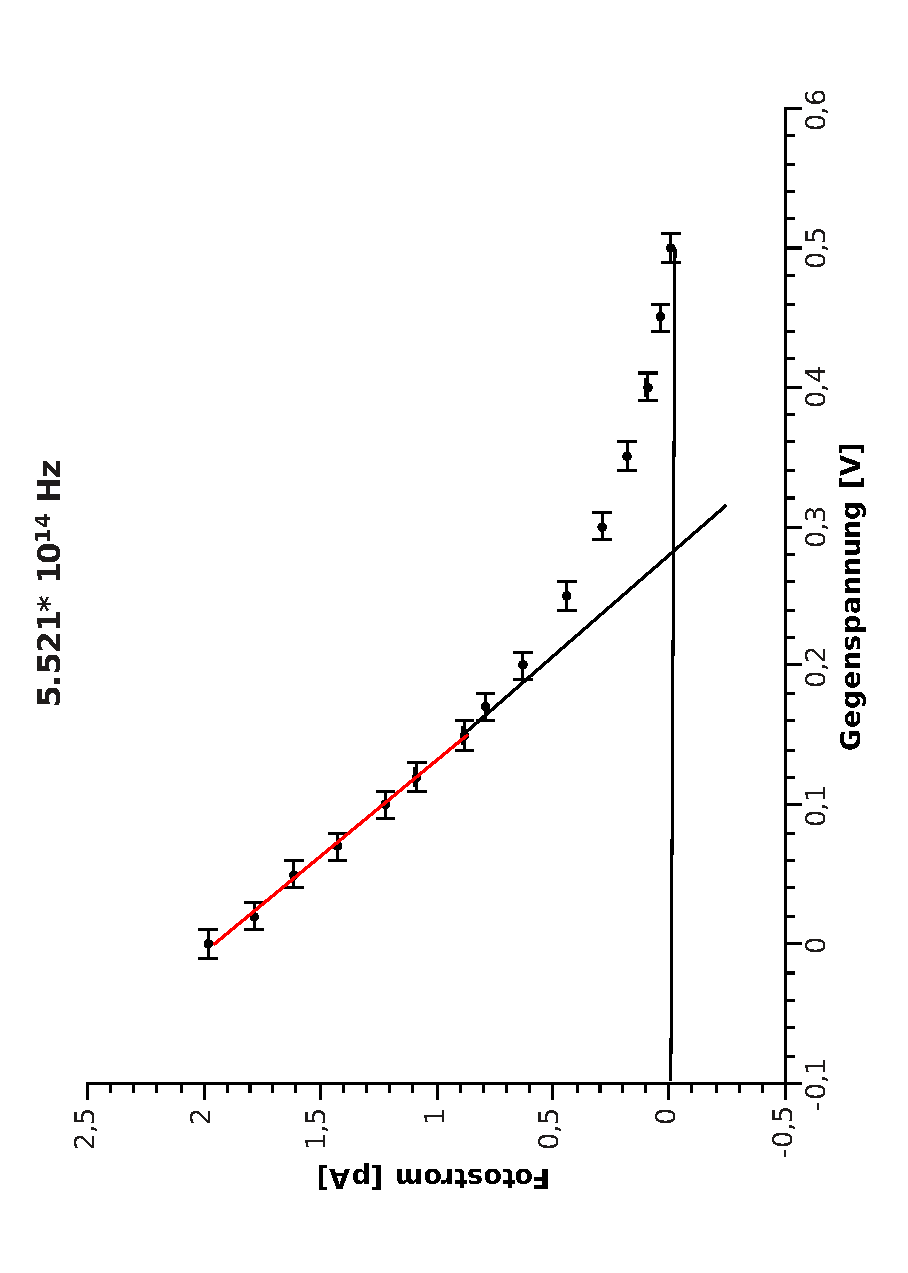
\includegraphics[width=0.75\linewidth, angle=-90]{5521.eps}
\end{subfigure}
\begin{subfigure}{0.48\textwidth}
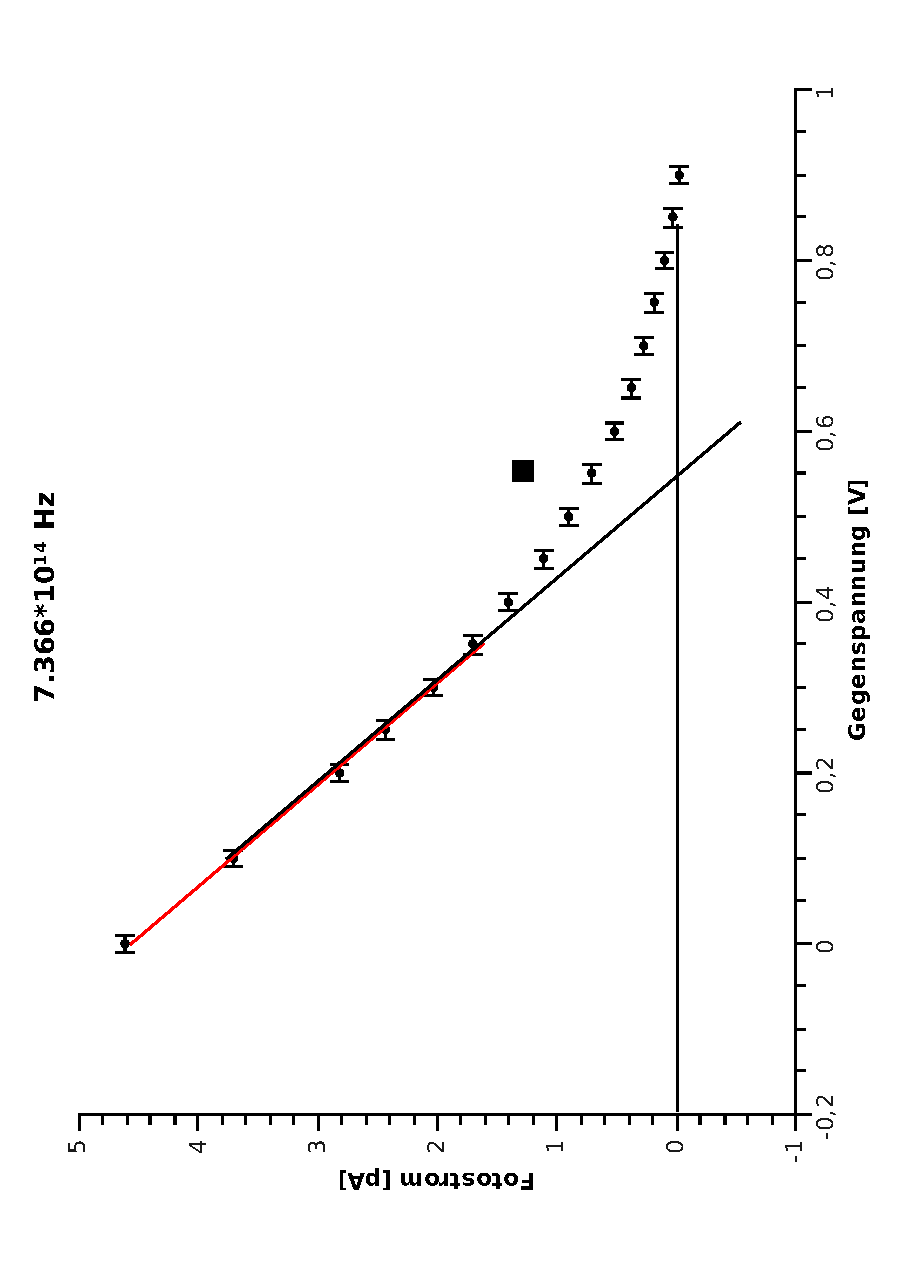
\includegraphics[width=0.75\linewidth, angle=-90]{7366.eps}
\end{subfigure}
\begin{subfigure}{0.48\textwidth}
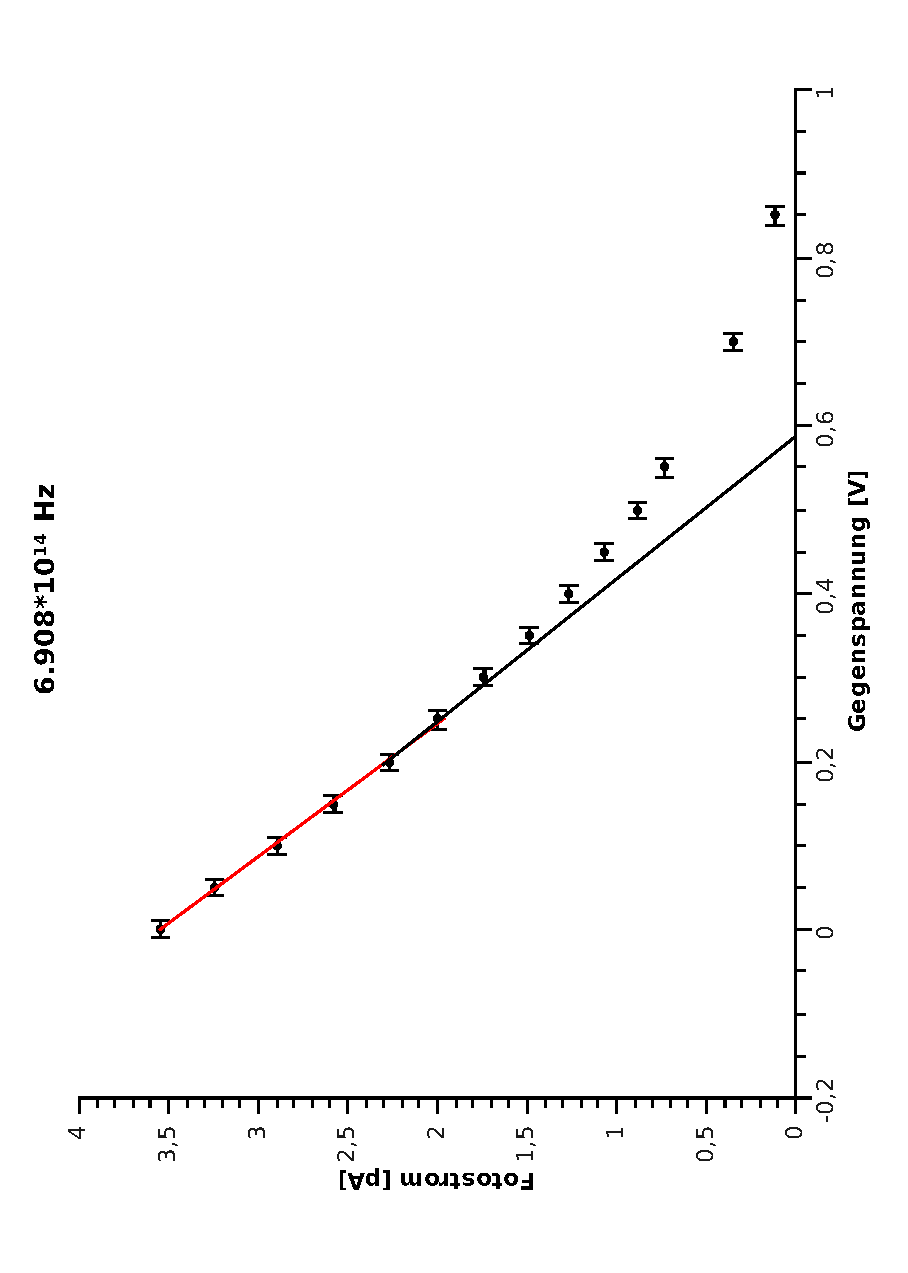
\includegraphics[width=0.75\linewidth, angle=-90]{6908.eps}
\end{subfigure}
\begin{subfigure}{0.48\textwidth}
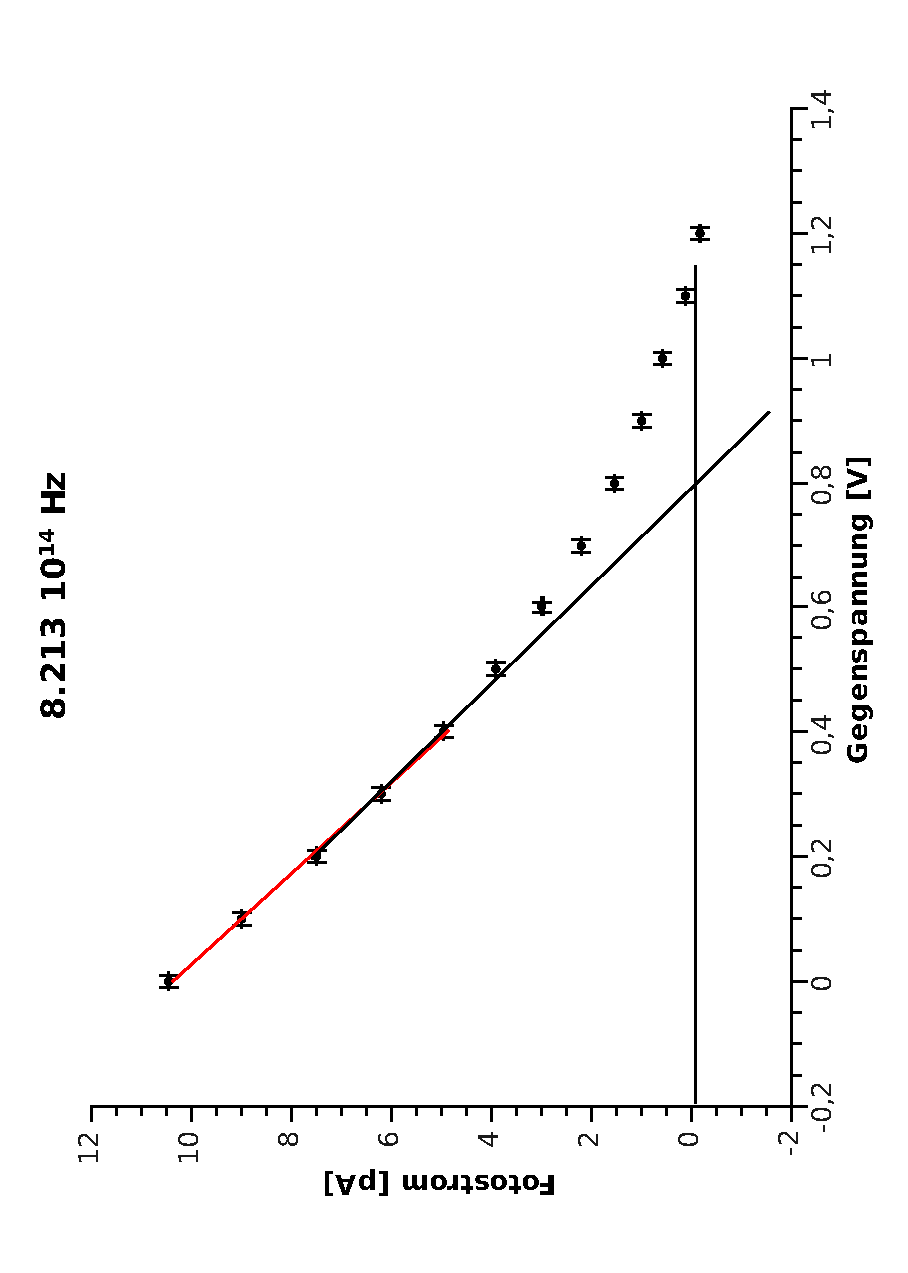
\includegraphics[width=0.75\linewidth, angle=-90]{8213.eps}
\end{subfigure}
\caption{Datenpunkte und Fits der anderen vier Frequenzen.}
\end{figure}
\end{center}

\newpage
Nun können wir einen  Plot erstellen, in dem die Spannung $U_0$ gegen die Frequenz $\nu$ aufgetragen ist. Wir sehen dabei, dass die Gerade nicht alle Datenpunkte miteinschließt. Da die Unsicherheiten bei den letzten Werten sehr gering sind (aufgrund des guten linearen Fits im ersten Schritt), versuchen wir es mit größeren Unsicherheiten:
\begin{center}
\begin{figure}[H]
\includegraphics[scale=0.75]{frequenz-spannung-unterschied.eps}
\caption{Spannung $U_0$ gegen Frequenz $\nu$ mit zwei unterschiedlichen linearen Fits für verschieden große Unsicherheiten. Dunkle Linie: Original-Unsicherheiten aus der obigen Tabelle. Helle Linie: Vergrößerte Unsicherheiten, die auch im Plot eingezeichnet sind.}
\end{figure}
\end{center}

Offensichtlich ändert sich die Steigung schon in einem gut sichtbaren Maße, wenn nur die Unsicherheiten der letzten drei Werte verdoppelt werden ($0.02$ statt $0.01$).\\
\\
Aus der Einstein-Formel 
$$h\cdot\nu=A+E_{kin}=A+eU_0$$
können wir die Austrittsarbeit $A$ und das Planck'sche Wirkungsquantum $h$ bestimmen. Umgeformt erhalten wir
$$U_0=\frac{h\cdot\nu}{e} - \frac{A}{e}$$
Die Regressionsgerade im obigen Plot entspricht genau dieser Gleichung. Wir erhalten also $h/e$ als die Steigung der Gerade, sowie $A/e$ als den Schnittpunkt mit der y-Achse.

Für die erste Gerade (dunkle Linie) erhalten wir die Werte: $h/e=0.17 \pm 0.01$ und $A/e=-0.64 \pm 0.08$. Für die zweite Gerade (helle Linie): $h/e=0.18 \pm 0.01$ und $A/e=-0.71 \pm 0.06$.\\
Mit $e=1.602177 \cdot 10^{-19}C$ und wenn wir bedenken, dass $\nu$ in $10^{14}$Hz gegeben war, erhalten wir:

$$\boxed{h=(2.85 \pm 0.03)\cdot 10^{-34}Js}$$
$$\boxed{A=(1.08 \pm 0.06)\cdot 10^{-19}Js=(1.08 \pm 0.06)eV}$$


%Gerade für $\nu=5.187$\\
%$Ax+B=(-2.1 \pm 0.1)x+(0.57 \pm 0.01)$\\
%%R^2=0.989
%$x=0.27 \pm 0.05$\\ %0.05
%$Ax+B=(-2.2 \pm 0.1)x+(0.58 \pm 0.01)$\\
%%R^2=0.992
%$x=0.26 \pm 0.05$\\
%(mit einem Fit-Punkt weniger)\\
%\\
%Gerade für $\nu=5.521$\\
%$(-7.0 \pm 0.2)x + (1.94 \pm 0.02)$\\
%$x=0.28 \pm 0.03$\\ %Gauß: $\pm 0.03037$
%%R^2=0.995
%$(-7.2 \pm 0.2)x + (1.95 \pm 0.02)$\\
%$x=0.27 \pm 0.03$\\ %Gauß: $\pm 0.0296$
%%R^2=0.996
%\\
%Gerade für $\nu=6.908$\\
%$(-8.39 \pm 0.01)x + (4.5637 \pm 0.0008)$\\
%$x=0.5439 \pm 0.001$\\
%%R^2=0.997
%$(-8.62 \pm 0.01)x + (4.5874 \pm 0.0008)$\\
%$x=0.532181 \pm 0.001$\\
%%R^2=0.999
%
%Gerade für $\nu=7.366$\\
%$(-5.94 \pm 0.01)x + (3.50866 \pm 0.0006)$\\
%$x=0.59068 \pm 0.0017$
%%R^2=0.996
%$(-6.11 \pm 0.01)x + (3.525857 \pm 0.0007)$\\
%$x=0.577063 \pm 0.0016$
%%R^2=0.997
%
%Gerade für $\nu=8.213$\\
%$(-13.17 \pm 0.01)x + (10.3019 \pm 0.0007)$
%$x=0.782 \pm 0.001$
%%R^2=0.996
%$(-13.76 \pm 0.01)x + (10.38 \pm 0.001)$
%$x=0.754 \pm 0.001$
%%R^2=0.998

%Bestimmen Sie zu jeder Frequenz (Wellenlänge) die Gegenspannung $U_0$, bei der die schnellsten Elektronen den Anodenring gerade nicht mehr erreichen.
%Stellen Sie in einem Diagramm die Gegenspannung $U_0$ gegen die Frequenz $\nu$ dar. Führen Sie ein lineare Regression durch und bestimmen Sie die Austrittsarbeit $A$ und das Planck'sche Wirkungsquantum $h$. Entnehmen Sie aus dem Diagramm bei $U_0=0$ die untere Grenzfrequenz $\nu_g$.

%Stellen Sie entsprechend der Einsteingleichung die Spannung $U_0$ als Funktion der Frequenz $\nu$ graphisch dar und bestimmen Sie das Planck'sche Wirkungsquantum $h$, die Austrittsarbeit $A$ der Fotokathode und die untere Grenzfrequenz $\nu_g$.



\subsection{Wärmestrahlung}
%Tragen Sie in einem Diagramm die der Beleuchtungsstärke proprotionale Spannung in mV gegen $\frac{1}{r^2}$ für zwei Betriebsbedingungen (vom Betreuer erfragen) der Glühlampe auf. 14

%Abstand Ablesemarke - strahlende Fläche: $38\pm 1 \si{mm}$\\
%Abstand Ablesemarke - Fotozelle: $17.5 \pm 0.5 \si{mm}$\\
%Der Abstand r soll den Wert 50cm nicht unterschreiten.\\
Modus A: \begin{center}

 \fbox{$I=(3.82 \pm 0.01)\si{A}$ \hspace{8mm} $U=(3.65 \pm 0.01)\si{V}$}\\

Daraus berechnet:\\
 \fbox{$P_1=U\cdot I = (13.94 \pm 0.06) \si{W}$}
 \end{center}
Modus C: \begin{center} \fbox{$I=(4.81 \pm 0.01)\si{A}$ \hspace{8mm} $U=(5.63 \pm 0.01)\si{V}$} \\

Daraus berechnet:\\
 \fbox{$P_2=U\cdot I = (27.08 \pm 0.08) \si{W}$}
\end{center}
Die Unsicherheiten wurden mittels der Gaußschen Fehlerfortpflanzung ermittelt.\\
\begin{table}[H]
\begin{center}
\begin{tabular}{|c|c|c|}
\hline
$r$ (cm) & $U_A$ (mV $\pm$ 1mV) & $U_C$ (mV $\pm$ 1mV)\\
\hline
97 & 49 & 259 \\
92 & 54 & 289 \\
87 & 59 & 321 \\
82 & 65 & 360 \\
77 & 75 & 410 \\
72 & 86 & 473 \\
67 & 100 & 553 \\
62 & 118 & 657 \\
57 & 142 & 793 \\
52 & 167 & 982 \\
\hline
\hline
\end{tabular}
\caption{Spannung an der Fotozelle und Abstände $r$ von der Glühlampe für zwei verschiedene Bestriebsbedingungen.}
\end{center}
\end{table}

%Bestimmen Sie die jeweils zugehörigen elektrischen Leistungen $P_1$ und $P_2$.

%Berechnen Sie für beide Betriebsbedingungen die Strahlungstemperaturen der Glühlampe. 12 und 13

\begin{figure}[H]
\centering
\begin{subfigure}{0.48\linewidth}
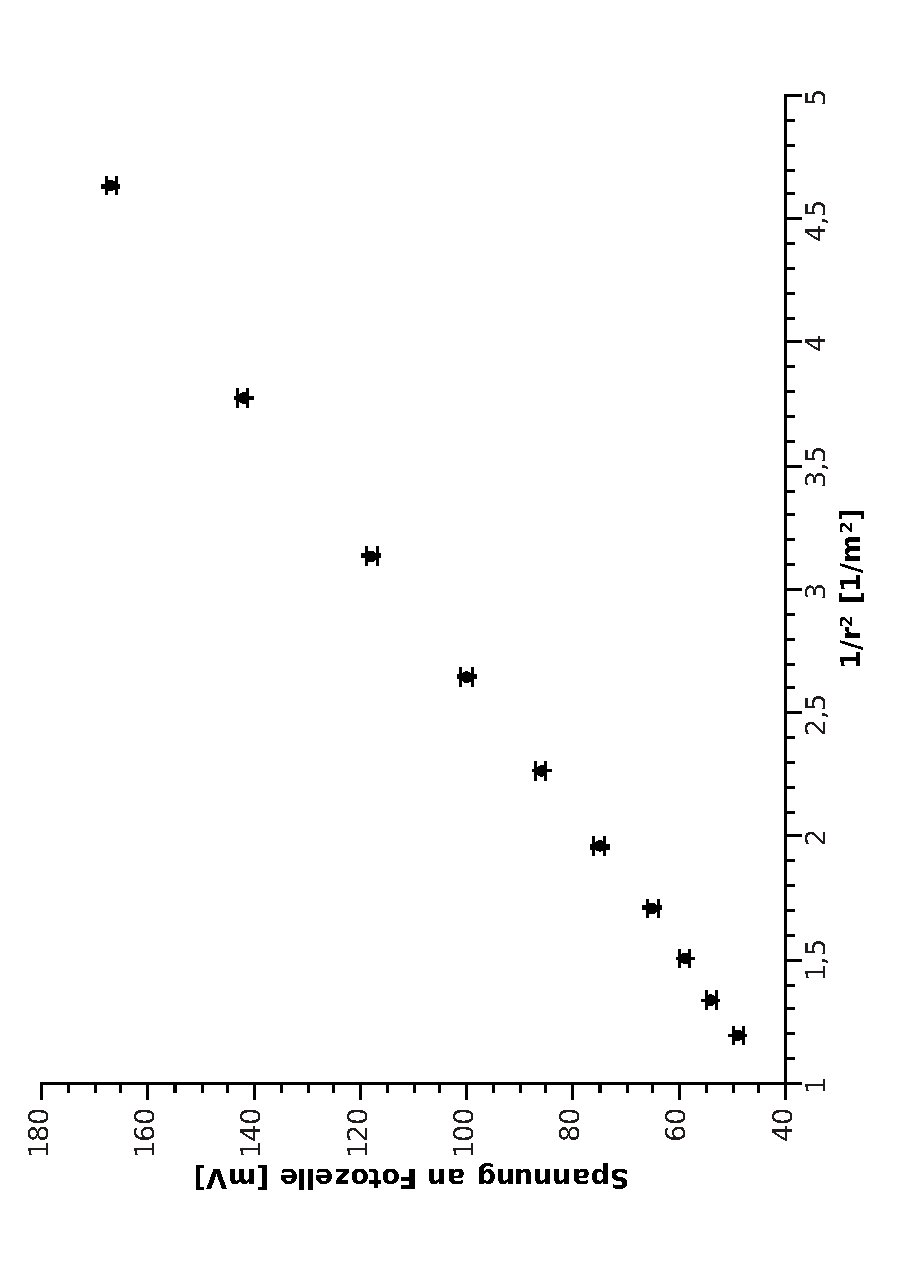
\includegraphics[width=0.75\linewidth, angle=-90]{niedrigetemp.eps}
\caption{ \label{figLowTemp} Betriebsmodus A}
\end{subfigure}
\begin{subfigure}{0.48\linewidth}
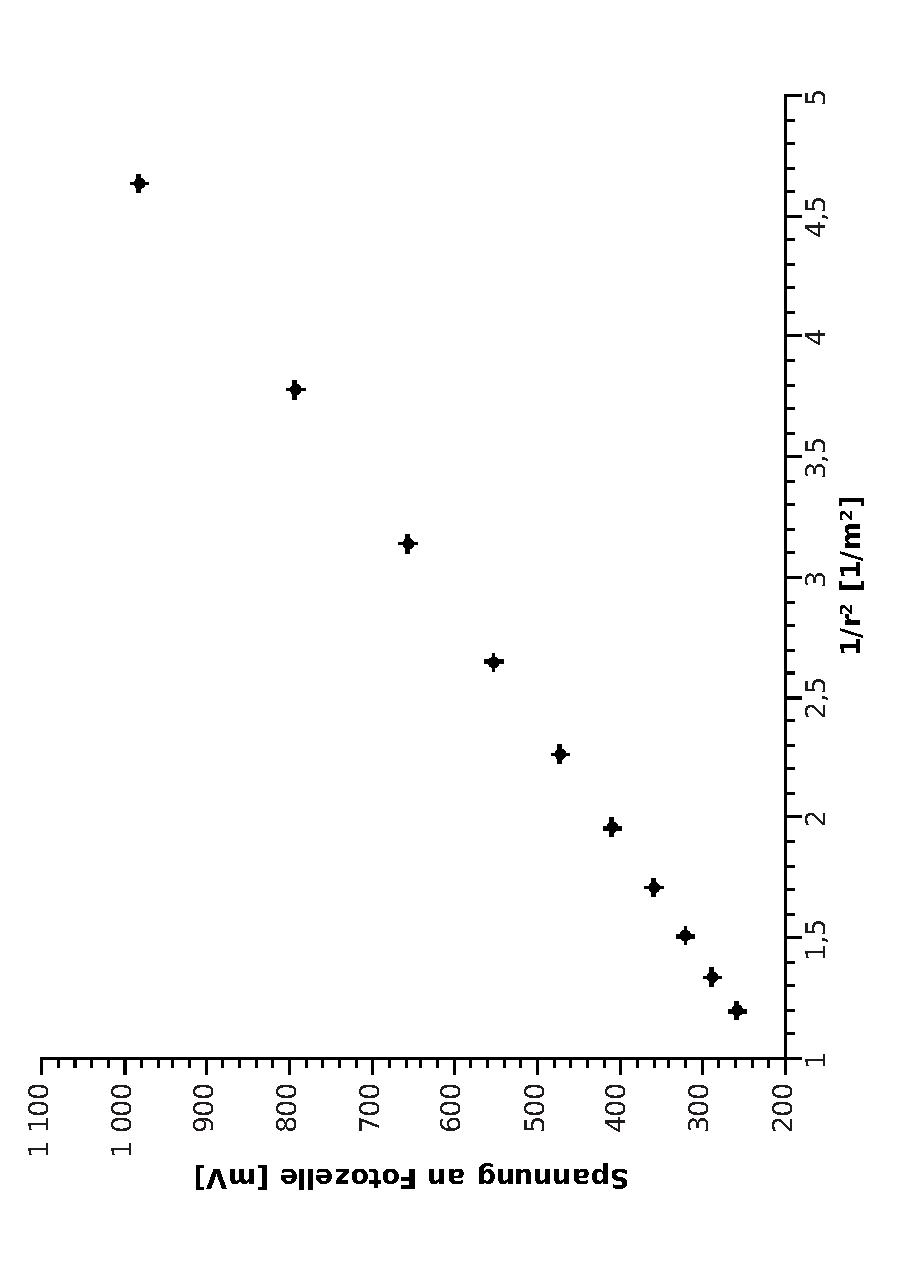
\includegraphics[width=0.75\linewidth, angle=-90]{hohetemp.eps}
\caption{Betriebsmodus \label{figHighTemp} C}
\end{subfigure}
\caption{Die der Beleuchtungsstärke proportionale Spannung an der Fotozelle, gegen das Inverse des Abstandsquadrates}
\end{figure}

Mittels linearer Fits wurden die Anstiege der Beleuchtungsstärken gegen die Inversen der Abstandsquadrate gewonnen:\\
\vspace{5mm}
\begin{center}
Für Abb. (\ref{figLowTemp}): \hspace{1cm}  (35,15 $\pm$ 0,30 ) \\
Für Abb. (\ref{figHighTemp}): \hspace{1cm} (209,55 $\pm$ 0,30) \\
\end{center}
\vspace{5mm}
Wir verwenden diese Werte nun als $r_1^2$ und $r_2^2$ in den Formeln (\ref{waermetheorie}) bis (\ref{waermeende}) und ermitteln die Temperaturen der Lampe: \\
\begin{center}
$T_1=2201.4 K$ \\
Wir berechnen $T_2$ aus $T_1$: \\
\begin{equation}
T_2=\frac{T_1}{\sqrt[4]{\frac{P_1}{P_2}}} 
\end{equation}
$T_2=2599.0 K$ \\
\end{center}
Wir beginnen eine Fehlerfortpflanzungsorgie, auf deren Methode wir in der Diskussion eingehen:
\begin{align*}
&I_{rel}=\frac{I_1}{I_2}\\
&\Delta I_{rel}=\sqrt{ \left(\frac{\delta I_{rel}}{\delta r_1^2}\right)^2 \cdot \Delta (r_1^2)^2 + \left(\frac{\delta I_{rel}}{\delta r_2^2}\right)^2 \cdot \Delta (r_2^2)^2 } = 0.0014156 \\
&\Delta ln (I_{rel})= \frac{1}{2} \cdot ( ln(I_{rel}+ \Delta I_{rel}) - ln ( I_{rel} - \Delta I_{rel}) ) =  0.00844\\
&P_{rel}=\frac{P_1}{P_2} \\
&\Delta P_{rel} = \sqrt{ \left(\frac{\delta P_{rel}}{\delta P_1}\right)^2 \cdot \Delta P_1^2 + \left(\frac{\delta P_{rel}}{\delta P_2}\right)^2 \cdot \Delta P_2^2)} =  0.0032 \\
&\Delta \sqrt[4]{P_{rel}} = \frac{1}{2} \left(  \sqrt[4]{P_{rel}+ \Delta P_{rel}} -\sqrt[4]{P_{rel}-\Delta P_{rel}} \right) = 0.0026 \\
&\Delta T_1 = \sqrt{ \frac{ (\Delta \sqrt[4]{P_{rel}})^2}{ln(I_{rel})^2} \cdot \left( \frac{c \cdot h}{k_B\cdot \lambda} \right) ^2 + \frac{ (\sqrt[4]{P_{rel}})^2 \cdot (\Delta ln(I_{rel}))^2}{ln(I_{rel})^4} \cdot \left( \frac{c \cdot h}{k_B \cdot \lambda}  \right) ^2} = \textbf{ 69 } ^{\circ} K \\
&\Delta T_2 = \sqrt{ \frac{ ( \Delta T_1)^2}{\sqrt{P_{rel}}} + \frac{T_1^2 \cdot ( \Delta \sqrt[4]{P_{rel}})^2}{16 \cdot P_{rel}^{\frac{6}{4}} } } = \textbf{ 82 } ^{\circ} K
\end{align*}
Daraus folgt als Endergebnis für die Temperaturen:
\begin{center}
\fbox{
$T_1=(2200 \pm 70) ^{\circ} K$}

\fbox{ 
$T_2=(2600 \pm 90) ^{\circ} K$}
\end{center}
\newpage
\section{Diskussion}
\subsection{Planck'sches Wirkungsquantum}
Der Literaturwert für $h$ beträgt $6.626 \cdot 10^{-34}Js$. Unser Wert weicht mit $h=(2.85 \pm 0.03)\cdot 10^{-34}Js$ um einen Faktor 2.3 davon ab, allerdings ist die Größenordnung passend. Wie oben bereits sichtbar, ändert schon allein die Größe der Unsicherheiten die Steigung der Gerade. Außerdem wirkt aufgrund der geringen Zahl an Messpunkten (wir hatten nur 5 Frequenz-Filter zur Verfügung) der letzte Wert als Hebel. Daraus erklären wir uns die Abweichung.\\
Die Austrittsarbeit $A=(1.08 \pm 0.06)eV$ können wir nicht so genau vergleichen, da wir nicht wissen, um welches Metall es sich bei der Kathode handelt und die Liste der Austrittsarbeiten von $1eV$ bis $5eV$ reicht. Wäre unser Wert für das Planck'sche Wirkungsquantum besser würden wir es uns erlauben, das Metall über die Austrittsarbeit zu bestimmen. So kann es aber leicht sein, dass auch unser gemessenes $A$ um einen Faktor 2 falsch ist.

\subsection{Wärmestrahlung}
Wir haben bei der Berechnung der Unsicherheit einen kleinen mathematischen Trick verwendet. Dabei haben wir den langen Ausdruck für $T_1$ nicht nach jeder einzelnen Messgröße abgeleitet, sondern erst die Unsicherheiten der zusammengesetzten Größen wie $\sqrt[4]{\frac{P_1}{P_2}}$ bestimmt und dann nach diesen abgeleitet. Außerdem haben wir zwei mal eine halbierte Größtfehlerabschätzung verwendet.   

Die Unsicherheiten der $r_i^2$ wurden in der Unsicherheit der linearen Fits berücksichtigt. Den größten Beitrag für die Unsicherheit der Temperaturen liefert die Unsicherheit der relativen Leistung, was vor allem durch die vierte Potenz im Nenner des Summanden in der Gaußschen Fehlerfortpflanzung, der die Unsicherheit der relativen Intenstität im Zähler trägt, verstärkt wird. \\
																							
\end{document}
